\documentclass[tikz,border=10pt]{standalone}
\usepackage{tikz}
\usetikzlibrary{shapes,arrows,positioning,calc,patterns,shadows,arrows.meta}

\definecolor{bertblue}{RGB}{66,133,244}
\definecolor{maskred}{RGB}{234,67,53}
\definecolor{tokencolor}{RGB}{142,36,245}
\definecolor{attentioncolor}{RGB}{52,168,83}

\begin{document}
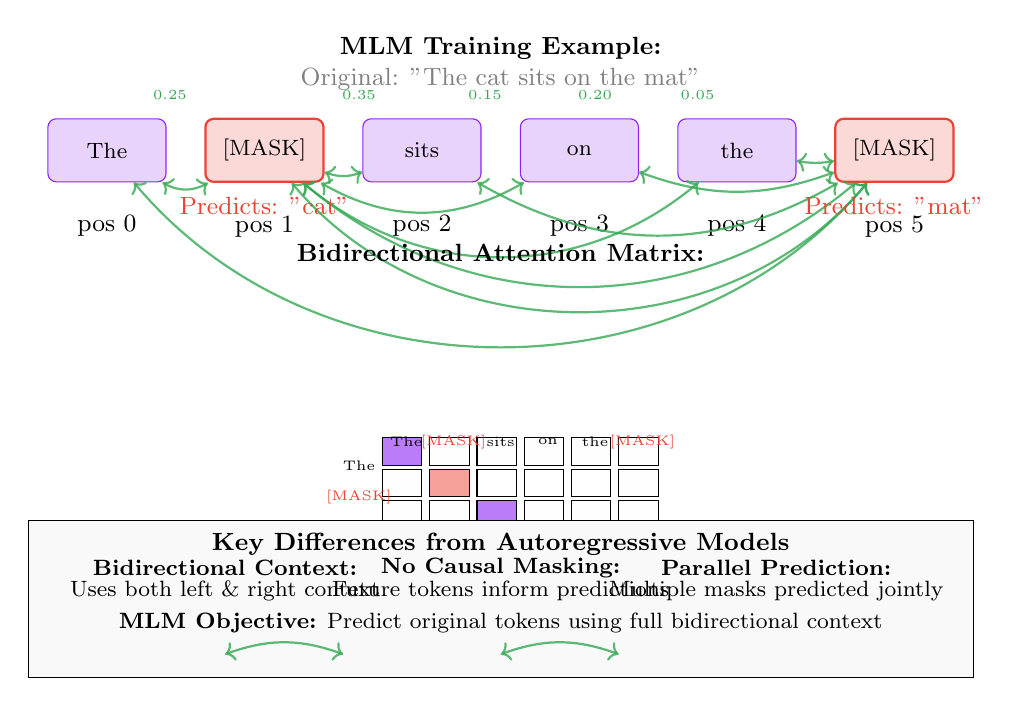
\begin{tikzpicture}[
    token/.style={rectangle, rounded corners=3pt, minimum width=1.5cm, minimum height=0.8cm, font=\footnotesize},
    masktoken/.style={token, fill=maskred!20, draw=maskred, thick},
    normaltoken/.style={token, fill=tokencolor!20, draw=tokencolor},
    attention/.style={<->, thick, attentioncolor, opacity=0.8},
    prediction/.style={->, very thick, maskred},
    label/.style={font=\small},
    title/.style={font=\large\bfseries}
]

% Title removed - using figure caption instead

% Input sequence with MASK
\node[label] at (6, 7.8) {\textbf{MLM Training Example:}};

% Original text
\node[label, gray] at (6, 7.4) {Original: "The cat sits on the mat"};

% Masked sequence
\node[normaltoken] (t1) at (1, 6.5) {The};
\node[masktoken] (mask1) at (3, 6.5) {[MASK]};
\node[normaltoken] (t3) at (5, 6.5) {sits};
\node[normaltoken] (t4) at (7, 6.5) {on};
\node[normaltoken] (t5) at (9, 6.5) {the};
\node[masktoken] (mask2) at (11, 6.5) {[MASK]};

% Position labels
\node[label, below=0.3cm of t1] {pos 0};
\node[label, below=0.3cm of mask1] {pos 1};
\node[label, below=0.3cm of t3] {pos 2};
\node[label, below=0.3cm of t4] {pos 3};
\node[label, below=0.3cm of t5] {pos 4};
\node[label, below=0.3cm of mask2] {pos 5};

% Bidirectional attention from first MASK
\draw[attention] (mask1) to[bend left=30] (t1);
\draw[attention] (mask1) to[bend right=20] (t3);
\draw[attention] (mask1) to[bend right=30] (t4);
\draw[attention] (mask1) to[bend right=40] (t5);
\draw[attention] (mask1) to[bend right=50] (mask2);

% Bidirectional attention from second MASK
\draw[attention] (mask2) to[bend left=50] (t1);
\draw[attention] (mask2) to[bend left=40] (mask1);
\draw[attention] (mask2) to[bend left=30] (t3);
\draw[attention] (mask2) to[bend left=20] (t4);
\draw[attention] (mask2) to[bend left=10] (t5);

% Attention weights for first MASK
\node[label, attentioncolor, font=\tiny] at (1.8, 7.2) {0.25};
\node[label, attentioncolor, font=\tiny] at (4.2, 7.2) {0.35};
\node[label, attentioncolor, font=\tiny] at (5.8, 7.2) {0.15};
\node[label, attentioncolor, font=\tiny] at (7.2, 7.2) {0.20};
\node[label, attentioncolor, font=\tiny] at (8.5, 7.2) {0.05};

% Predictions
\node[label, maskred] at (3, 5.8) {Predicts: "cat"};
\node[label, maskred] at (11, 5.8) {Predicts: "mat"};

% Attention matrix visualization
\node[label] at (6, 5.2) {\textbf{Bidirectional Attention Matrix:}};

\begin{scope}[shift={(6,2.5)}]
% Create 6x6 attention matrix
\foreach \i in {0,...,5} {
    \foreach \j in {0,...,5} {
        % Different patterns for MASK positions (1 and 5)
        \ifnum\i=1 % First MASK row
            \ifnum\j=1
                \fill[maskred!50] (\j*0.6-1.5, -\i*0.4) rectangle ++(0.5, 0.35);
            \else
                \pgfmathsetmacro{\weight}{0.6 + 0.1*cos(60*\j)}
                \fill[attentioncolor!\weight!white] (\j*0.6-1.5, -\i*0.4) rectangle ++(0.5, 0.35);
            \fi
        \else
            \ifnum\i=5 % Second MASK row
                \ifnum\j=5
                    \fill[maskred!50] (\j*0.6-1.5, -\i*0.4) rectangle ++(0.5, 0.35);
                \else
                    \pgfmathsetmacro{\weight}{0.5 + 0.15*cos(45*\j)}
                    \fill[attentioncolor!\weight!white] (\j*0.6-1.5, -\i*0.4) rectangle ++(0.5, 0.35);
                \fi
            \else % Normal token rows
                \ifnum\j=\i
                    \fill[tokencolor!60] (\j*0.6-1.5, -\i*0.4) rectangle ++(0.5, 0.35);
                \else
                    \pgfmathsetmacro{\weight}{0.3 + 0.1*cos(30*(\i+\j))}
                    \fill[blue!\weight!white] (\j*0.6-1.5, -\i*0.4) rectangle ++(0.5, 0.35);
                \fi
            \fi
        \fi
        \draw[thin] (\j*0.6-1.5, -\i*0.4) rectangle ++(0.5, 0.35);
    }
}

% Matrix labels
\node[label, font=\tiny] at (-1.8, 0) {The};
\node[label, font=\tiny, maskred] at (-1.8, -0.4) {[MASK]};
\node[label, font=\tiny] at (-1.8, -0.8) {sits};
\node[label, font=\tiny] at (-1.8, -1.2) {on};
\node[label, font=\tiny] at (-1.8, -1.6) {the};
\node[label, font=\tiny, maskred] at (-1.8, -2.0) {[MASK]};

\node[label, font=\tiny] at (-1.2, 0.3) {The};
\node[label, font=\tiny, maskred] at (-0.6, 0.3) {[MASK]};
\node[label, font=\tiny] at (0, 0.3) {sits};
\node[label, font=\tiny] at (0.6, 0.3) {on};
\node[label, font=\tiny] at (1.2, 0.3) {the};
\node[label, font=\tiny, maskred] at (1.8, 0.3) {[MASK]};
\end{scope}

% Key insights
\node[rectangle, draw=black, fill=gray!5, minimum width=12cm, minimum height=2cm] at (6, 0.8) {};
\node[label, font=\small\bfseries] at (6, 1.5) {Key Differences from Autoregressive Models};

% Bidirectional flow
\node[label, font=\footnotesize] at (2.5, 1.2) {\textbf{Bidirectional Context:}};
\node[label, font=\footnotesize] at (2.5, 0.9) {Uses both left \& right context};

% No causal masking
\node[label, font=\footnotesize] at (6, 1.2) {\textbf{No Causal Masking:}};
\node[label, font=\footnotesize] at (6, 0.9) {Future tokens inform predictions};

% Multiple predictions
\node[label, font=\footnotesize] at (9.5, 1.2) {\textbf{Parallel Prediction:}};
\node[label, font=\footnotesize] at (9.5, 0.9) {Multiple masks predicted jointly};

% MLM objective
\node[label, font=\footnotesize, align=center] at (6, 0.5) {\textbf{MLM Objective:} Predict original tokens using full bidirectional context};

% Attention flow arrows
\draw[attention, bend left=20] (2.5, 0.1) to (4, 0.1);
\draw[attention, bend right=20] (7.5, 0.1) to (6, 0.1);

\end{tikzpicture}
\end{document}